\chapter{Analýza a srovnání}

\section{Vymezení fyziologické schopnosti}
Když se zeptáme proč se někdo nějaký schopnost dokázal učit nebo ne musíme se zeptat jestli byly schopní se to naučit.  Protože děláme studium, který zabývá s citem hmatu, musíme najít omezení hmatu.

Abych zajistil, že můj FCHAD je fyzické použitelný jsem si přečetl kapitolu \em Haptic Interfaces\em  od knihy \em HCI Beyond the GUI\em. Člověk má šest druhů hmatových receptorů, volná nervová zakončení, Meissnerovo tělísko, Merkelova buňka, Paciniho tělíska, receptory vlasového folikulu, Ruffiniho tělíska. Různé hmatné receptory mají jiné citlivosti.  Například Paciniho tělíska cítí jenom vibrace.

Pro účelu FCHADu, chceme spustit receptory, které reagují rychle a přesně.  Myslím si, že je to taky lepší spouštět vice druhů receptorů ale nejsem si jistý.  Prostorově nejpřesnější receptory jsou Meissnerovo tělísko a Merkelova buňka.  Ty jsou dost hluboké v kůže, proto používáme silné pohyblivé solenoidy.  Druhý verze FCHADu taky produkuje malou vibrace o 200Hz což je doporučený frekvence v publikace HCI\citep[str. 29-30]{nielsen2008gesture}.

Autoři samy kapitole rozdělí čtyři subjektivní druhy hmatu: tlak, dotyk, vibrace a lechtání.  Myslím si, že lechtání se produkuje pohybem přes prsti.  Jeden hypotéza proč FCHADy nefungují moc dobře je, že pohyb bodů na prstech pomůže čtenář rozpoznat písmeno.  Christophe Ramstein v 1996 studie píše o FCHADech: \em \uv{Protože vice mechanorecoptorů jsou použití v hmatovém vnímání, pohyb prstu nad tvarem anebo zrnitosti zlepšuje vnímání.  V případě jedno-písmenové zobrazovače důsledkem je, že prst necítí přechod mezi písmenem ale jen změna uspořádání.  Protože prst nechybuje, rychlost je pomalejší než s 20ti, 40ti, anebo 80ti písmenová zobrazovače(46.1 slov za minut u rychlé čtenáři a 12.0 slov za minut pro pomalé čtenáři} \em \citep[str. 38, přeložený z angličtiny]{ramstein1996combining}
%"Because multiple mechanical receptors are involved in the tactile perception mechanism, the displacement of the finger over a form or texture improves perception and facilitates acknowledgement[7,14]. As a result, in the single cell case, the finger will not feel the transition from one character to the next, but only the configurational changes in the cell’s pins according to the following character.  Since the finger is not moving on the braille characters, speed performance will of course be slower than on 20-, 40- or 8O-cell braille displays (46.1 wpm for fast readers and 12.0 wpm for slow readers)."
Když si čtu tisknutá Braillova písma se cítím, že je to určitý druh lechtání.  Abych přidal podobnou pocit u zobrazovače FCHADu dal jsem kus látky nad zobrazovačem.  Líbilo mě to ale nepoužíval jsem tu látku v studie. Myslel jsem si, že by věci jenom zkomplikovali pro moje účastnici.

Publikace HCI sestavuje pro naše použity prahy rozlišený anebo v angličtině "Just Noticeable Differences(JND)". Neberu JNDy jako měřítku to co člověk dokáže cítit, ale spíš co nedokáže.  Nechtěl jsem aby nastroj pracoval na hranice citlivosti ale aby znaky byly bezpečně rozpoznatelné.

Pocit hmatu je přesný do ${}1mm^2 - 2mm^2$ na konce prstů a až ${}45mm^2$ jinde na tělo.  Tisknutí Braillovo písmo má body vzdálené od sebe 2.3-2.5mm\citep{brailleauthority}. To je až příliš blízko JND.  Však Perkins produkuje speciální velko-písmenové psací stroj kvůli tomu, že některé nevidomé nedokážou normální Braillovo písmo číst\footnote{\url{https://secure2.convio.net/psb/site/Ecommerce?FOLDER=1180&store_id=1101&JServSessionIdr004=9p1uhglug2.app246a&__utma=184864936.426189431.1365936556.1365946389.1366050996.3&__utmb=184864936.1.10.1366050996&__utmc=184864936&__utmx=-&__utmz=184864936.1365936556.1.1.utmcsr=(direct)|utmccn=(direct)|utmcmd=(none)&__utmv=-&__utmk=194396717}}.  Bohužel, když děláme větší písmo už to nevejde na koncem prstu a kůže jinde na tělo je méně citlivá.  Vzdálenost JND kůže na dlaně je 11mm a proto, hrozí se že zvětšení písmo zhoršuje čtení! Můj osobní pocit je, že optimální velikost pro Braillovo písmo je 500 x 300mm.  Když jsem vyrobil první FCHAD jsem nemohl dostat solenoidy tak malé, a proto v studie používal jsem daleko větší zobrazovač\citep[str. 30-32]{nielsen2008gesture}.

Další práh rozlišený je časový.  To není jen jak rychle něco cítíte ale kolik krát můžete něco cítit za sekund.  V angličtině "successiveness limen(SL)" je minimální čas dvě impulsy mohou mít aby člověk je rozlišil od sebe.  V našem studie žádný účastník nečetl tak rychle aby pobližil SL.  Stejně doufal jsem, že budou čist rychlejší, a doufám, že bude možní na FCHADu číst tak rychle jako tisknutí Braillovo písmo.  To je asi 7.9CPS\citep{wetzel2006studies}.  To znamená, že za každý 126ms musí čist jedno písmeno.  SL pro mechanoreceptory je 5 ms ale nás zajímá 20 ms, který je minimální čas aby člověk dvě pocity rozlišil ve správném pořady\citep[str. 32]{nielsen2008gesture}.

Další omezenost je absolutní velikost ruky.  Jestli ruka není dost velká nepokrývá celou zobrazovače.  Několik účastníků měli ruce dost malé aby nepokrývali zobrazovače pohodlně nikdo to nezvládl.

V závěru bych řekl, že účastnici studie byly fyzické schopní používat FCHAD správně a že citové hranici nehráli role v studie.


\section{Analýza rychlosti}
Kdyby to bylo čistě psychologické studium bych omezoval svůj vlastní přítomnost v zájmů srovnatelnost výsledků.  Dano, že to je pedagogický výzkum Já jsem jako pedagog a badatel nedělitelný součást výsledků.

Nemůžeme koukat na rychlost čtení a křivky učení jako absolutní hodnoty v této studiu protože rychlost čtení je ovlivněn do velké míru to, jestli jsem Já rozhodl něco prodlouženě vysvětlit nebo ne, a jestli Já jsem si rozhodl nechat chybu byt anebo ji upravit.

Kvůli velké potíže s čtení, žák 8 je z toho analýzu vynechán.

\paragraph{Jak čtete grafy?}  Grafy ukazují, který senzor byl vybraný v daném časů.  Kdy nebyl žádný senzor vybraný, je nakreslen stejným způsobem jako když 11ti senzor je vybraný.  Škále není normalizované. Číslo na pod grafem jsou absolutní čas.  Když graf je podznačení jako 22m a je napsáno 20-Mar-13 12:00 to znamená v 12:22 3.4.2013 a NE 22m po začátku studii.  Kdy čára vypadá \uv{chlupatý}, znamená, že byl špatný kontakt mezi prstem a senzorem.

Není smysluplný analyzovat časy čtení první řádku protože jsem tak často pomohl účastnicí a protože je kratší než ostatní.

% 3 = down 4 = up

\subsection{Žák 5}
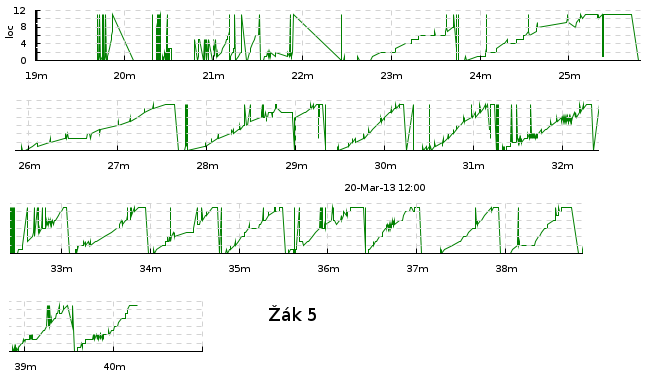
\includegraphics[width=1\textwidth]{Location5-cut}

Četl 17 řádků a jsou 17 trojúhelníky na grafu tak všechno je dobrý.

Uvažoval jsem dlouho jak měřit rychlost čtení na FCHADu.  Sice mám hezké grafy ale neznamená to, že mohu měřit přesní rychlost čtení.  Nezpracování data pro první tří písmena druhý řádek je například(trojtečky jsem dal, kde byly změní dotykovaných senzorů ale se zobrazené písmeno nezměnilo):
\begin{verbatim}
2013-03-20@12:23:44.436 Dolu  1 0 0 0 0 0 0 0 0 0 0 0 0 'k'
...
2013-03-20@12:23:49.634 Dolu  1 1 1 0 0 0 0 0 0 0 0 0 0 'k'
2013-03-20@12:23:49.964 Nahoru  0 1 1 0 0 0 0 0 0 0 0 0 1 'ý'
2013-03-20@12:23:50.129 Nahoru  0 1 0 0 0 0 0 0 0 0 0 0 1 'ý'
2013-03-20@12:23:50.212 Dolu  0 1 1 0 0 0 0 0 0 0 0 0 1 'ý'
2013-03-20@12:23:50.748 Dolu  1 1 1 0 0 0 0 0 0 0 0 0 0 'k'
2013-03-20@12:23:58.084 Nahoru 0 1 1 0 0 0 0 0 0 0 0 0 1 'ý'
2013-03-20@12:24:03.483 Dolu  0 1 1 1 0 0 0 0 0 0 0 0 1 'ý'
2013-03-20@12:24:03.525 Nahoru  0 0 1 1 0 0 0 0 0 0 0 0 2 ' '
\end{verbatim}
...
\begin{verbatim}
2013-03-20@12:24:11.233 Dolu  0 0 1 1 1 0 0 0 0 0 0 0 2 ' '

\end{verbatim}

Nuly a jedny naznačují jestli senzor byl dotýkaný. Například, řádek:
\begin{verbatim}
2013-03-20@12:24:11.233 Dolu  0 0 1 1 1 0 0 0 0 0 0 0 2 ' '
\end{verbatim}

znamená, že v 12:24:11.233 byl nový dotyk na pátý senzor, a že se zobrazovala mezera.  Jestli koukáte na čas 12:23:50.212 začíná se `ý' byt zobrazeno, ale v 12:23:50.748 se vrátil na `k'.  Není jasný, z toho kdy čtení jednoho písmeno končí a kdy čtený druhý začíná.  Celá sbírka dat je takhle rozmazaná.  Proto jsem si vybral způsob analýzou očima a s kružítkem.

Pátý žák se značně zrychlil během naše setkání.

První pět řádky se zrychlil každým řádkem ale mezi pátým řádkem a šestým řádkem není rozdíl v rychlosti. Sedmi řádek četl zase pomaleji ale osmi řádek byl jeho nejrychlejší řádek a četl rychleji než i pátý a šestý.  Devátý řádek zase četl stejně rychle jako pátý.  A desátý řádek zpomalil.  Zbytek času či zrychlil anebo zpomalil ale nelze poznat sklon.

\subsection{Žák 6}
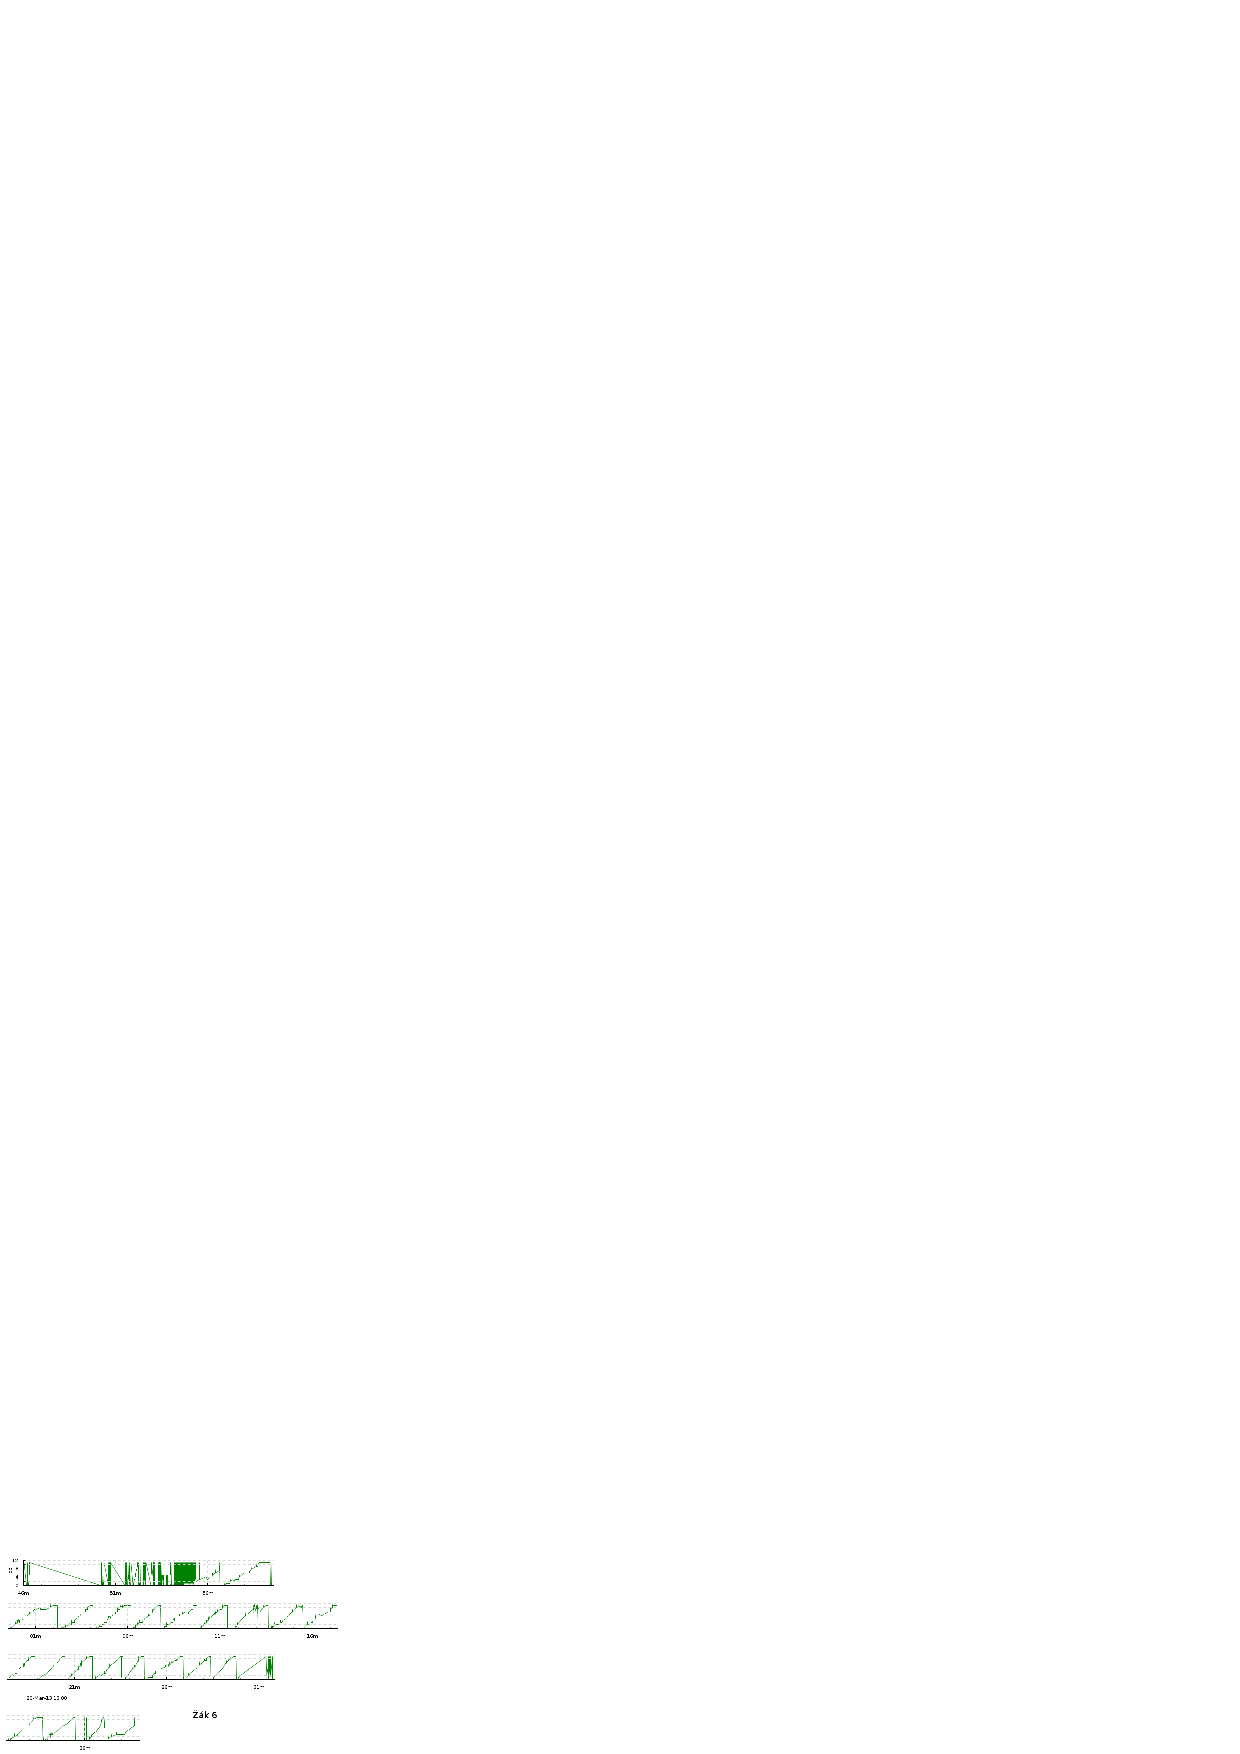
\includegraphics[width=1\textwidth]{Location6-cut}

Četla 22 řádků ale poslední četla jenom první 7 znaků.  Jsou 24 trojúhelníků na grafu ale rovná čára kolem 31 minut 20ti trojúhelník není čtení a předposlední řádek četla dva krát.

Žák 6 taky zrychlila ale ne tak pravidelně jako u pátého žáka.

Druhý a třetí řádky četla stejně rychle.  Čtvrtý řádek četla rychlejší ale trochu zpomalila u pátého řádku. Už nebyl poznat sklon.  Mezi řádky 12 a 16 pomalu zrychlila ale řádek 17 je značně pomalejší.  Dále není poznat sklon.  Předposlední řádek, kde měla číst slova a ne písmena a četla podruhy četla značně rychlejší

\subsection{Žák 7}
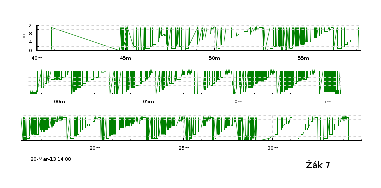
\includegraphics[width=1\textwidth]{Location7-cut}

Četl 19 řádků během setkání(ale četl desátý řádek dva krát a proto je na grafů dvacet trojúhelníků.

První čtyři řádky četl stejným rychlosti.  Odstranil prst z selektoru během čtení pátého řádku a proto vypadá rozdělené. Šesti řádek četl rychlejší než ty první ale jeho až na třinácti řádek, kde zase zrychlil.  Čtrnáctý řádek je pomalý, ale jinak zrychlil zbytek dobu čtení.


\subsection{Žák 9}
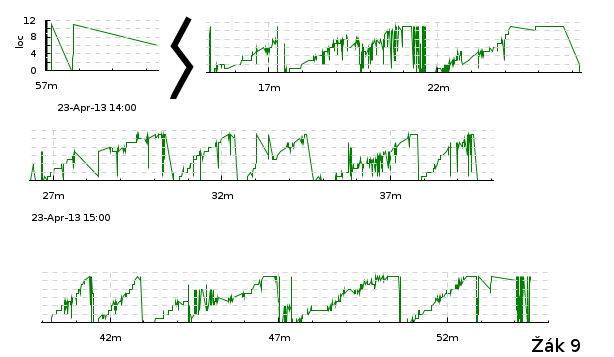
\includegraphics[width=1\textwidth]{Location9-cut}

Četl 13 řádků během setkání a jsou 13 trojúhelníků.

První čtyři řádky četl stejným rychlosti, pátý řádek byl rychlejší a šestý stejně rychle jako pátý. Sedmý je pomalý, ale osmi až desátý zrychlil.  Velké zpomalený u jedenáctého řádku je snad tím, že jsou tam čísla. A poslední dva řádky jsou pomalé protože používal selektor samostatně.

\subsection{Analýza chyb}

Tady jsou shromážděné chyby účastníků běžného studie.  Zase neuvedu tady výsledky osmi účastníka.

\begin{tabular}{|c|c|}
\hline
Symbol&Význam\\
\hline
NČ&Nečetl samostatně\\
\hline
??&Chyba, ale nebyla poznat jaký na nahrávce\\
\hline
>>&Přeskočil písmeno\\
\hline
*&Není poznat jestli byly chyby kvůli vádám audiu\\
\hline
!&Znak pro velké písmena\\
\hline
--&Četl s pomoci\\
\hline
\end{tabular}


%\paragraph{První Řádek}
\begin{tabular}{|c|c|c|c|c|c|c|c|c|c|c|c|c|}
\hline
Žák&B&r&a&i&l&l&s&&&&&\\
&\braillebox{1278}&\braillebox{1235}&\braillebox{1}&\braillebox{24}&\braillebox{123}&\braillebox{123}&\braillebox{234}&\braillebox{}&\braillebox{2358}&\braillebox{123}&\braillebox{}&\braillebox{}\\
\hline
5&&NČ&NČ&s&&&&>>&>>&>>&>>&>>\\
&&&&\braillebox{234}&&&&&&&&\\
\hline
6&v&&&&??&&&>>&>>&>>&>>&>>\\
&\braillebox{1236}&&&&&&&&&&&\\
\hline
7&ě&h&&,&&>>&&>>&>>&>>&>>&>>\\
&\braillebox{126}&\braillebox{125}&&\braillebox{2}&&&&&&&&\\
\hline
9&NČ&--&&&&&p&>>&>>&>>&>>&>>\\
&&&&&&&\braillebox{1234}&&&&&\\
\hline
\end{tabular}

%\paragraph{Druhý Řádek}
\begin{tabular}{|c|c|c|c|c|c|c|c|c|c|c|c|c|}
\hline
Žák&k&ý& &ř&á&d&e&k&,& &k&t\\
&\braillebox{1378}&\braillebox{12346}&\braillebox{}&\braillebox{2456}&\braillebox{16}&\braillebox{145}&\braillebox{15}&\braillebox{13}&\braillebox{2}&\braillebox{}&\braillebox{13}&\braillebox{2345}\\
\hline
5&&&&&&&&&NČ&&&\\
\hline
6&a&?p?&&?t?&&&??&&NČ&&&j\\
&\braillebox{1}&\braillebox{1234}&&\braillebox{2345}&&&&&&&&\braillebox{245}\\
\hline
7&&&&&&&&&&&&\\
\hline
9&&&&&&&&&&&a&\\
&&&&&&&&&&&\braillebox{1}&\\
\hline
\end{tabular}

%\paragraph{Třetí Řádek}
\begin{tabular}{|c|c|c|c|c|c|c|c|c|c|c|c|c|}
\hline
Žák&e&r&ý& &t&e&ď& &p&o&u&ž\\
&\braillebox{1578}&\braillebox{1235}&\braillebox{12346}&\braillebox{}&\braillebox{2345}&\braillebox{15}&\braillebox{1456}&\braillebox{}&\braillebox{1234}&\braillebox{135}&\braillebox{136}&\braillebox{2346}\\
\hline
5&&&&&&??&&&&&&\\
\hline
6&&&&&&&&&&r&&\\
&&&&&&&&&&\braillebox{1235}&&\\
\hline
7&&&&&&o&&&&k&&\\
&&&&&&\braillebox{135}&&&&\braillebox{13}&&\\
\hline
9&&&&&&&&&&&&z\\
&&&&&&&&&&&&\braillebox{1356}\\
\hline
\end{tabular}

%\paragraph{Čtvrtý Řádek}
\begin{tabular}{|c|c|c|c|c|c|c|c|c|c|c|c|c|}
\hline
Žák&í&v&á&t&e&,& &n&e&n&í& \\
&\braillebox{3478}&\braillebox{1236}&\braillebox{16}&\braillebox{2345}&\braillebox{15}&\braillebox{2}&\braillebox{}&\braillebox{1345}&\braillebox{15}&\braillebox{2345}&\braillebox{34}&\braillebox{}\\
\hline
5&&&&j&&&&d&&&&\\
&&&&\braillebox{245}&&&&\braillebox{145}&&&&\\
\hline
6&&l&&&&&&&&&&\\
&&\braillebox{123}&&&&&&&&&&\\
\hline
7&&&u&&o&&&d&&&&\\
&&&\braillebox{136}&&\braillebox{135}&&&\braillebox{145}&&&&\\
\hline
9&á&&&&i&&&ž(NČ)&>>&>>&t,á&\\
&\braillebox{16}&&&&\braillebox{24}&&&\braillebox{2346}&&&\braillebox{2345},\braillebox{16}&\\
\hline
\end{tabular}

%\paragraph{Pátý Řádek}
\begin{tabular}{|c|c|c|c|c|c|c|c|c|c|c|c|c|}
\hline
Žák&p&r&v&n&í& &ř&á&d&e&k&,\\
&\braillebox{123478}&\braillebox{1235}&\braillebox{1236}&\braillebox{1345}&\braillebox{34}&\braillebox{}&\braillebox{1235}&\braillebox{16}&\braillebox{145}&\braillebox{15}&\braillebox{13}&\braillebox{2}\\
\hline
5&&&&&&&&&&&&\\
\hline
6&&&&&&&&&&&a&NČ\\
&&&&&&&&&&&\braillebox{1}&\\
\hline
7&&&&&&*&*&*&*&*&*&*\\
\hline
9&&&&&&&&í&&&a&\\
&&&&&&&&\braillebox{34}&&&\braillebox{1}&\\
\hline
\end{tabular}

%\paragraph{Šestý Řádek}
\begin{tabular}{|c|c|c|c|c|c|c|c|c|c|c|c|c|}
\hline
Žák& &k&t&e&r&ý& &z&o&b&r&a\\
&\braillebox{78}&\braillebox{13}&\braillebox{2345}&\braillebox{15}&\braillebox{1235}&\braillebox{12346}&\braillebox{}&\braillebox{1356}&\braillebox{135}&\braillebox{12}&\braillebox{1235}&\braillebox{1}\\
\hline
5&&&&&&&&&&&&\\
\hline
6&&&&&&&&&&&&\\
\hline
7&&&&&&&&ř&&&&\\
&&&&&&&&\braillebox{2456}&&&&\\
\hline
9&&&&&&&&n&&&h&\\
&&&&&&&&\braillebox{1345}&&&\braillebox{125}&\\
\hline
\end{tabular}

%\paragraph{Řádek 7}
\begin{tabular}{|c|c|c|c|c|c|c|c|c|c|c|c|c|}
\hline
Žák&z&u&j&e& &j&e&n&o&m& &j\\
&\braillebox{135678}&\braillebox{136}&\braillebox{245}&\braillebox{15}&\braillebox{}&\braillebox{245}&\braillebox{15}&\braillebox{1345}&\braillebox{135}&\braillebox{134}&\braillebox{}&\braillebox{245}\\
\hline
5&&&&&&&&&&&&\\
\hline
6&&&&&&&&d&&&&\\
&&&&&&&&\braillebox{145}&&&&\\
\hline
7&&&&&&&&&&&&\\
\hline
9&n&a&h&&&h&&d&&k&&,\\
&\braillebox{1345}&\braillebox{1}&\braillebox{125}&&&\braillebox{125}&&\braillebox{145}&&\braillebox{13}&&\braillebox{2}\\
\hline
\end{tabular}

%\paragraph{Řádek 8}
\begin{tabular}{|c|c|c|c|c|c|c|c|c|c|c|c|c|}
\hline
Žák&e&d&n&o& &p&í&s&m&e&n&o\\
&\braillebox{1578}&\braillebox{145}&\braillebox{1345}&\braillebox{135}&\braillebox{}&\braillebox{1234}&\braillebox{34}&\braillebox{234}&\braillebox{134}&\braillebox{15}&\braillebox{1345}&\braillebox{135}\\
\hline
5&&&&&&&&&&&&\\
\hline
6&&&&&&&&&&&&\\
\hline
7&&&&&&&&??&&&&a\\
&&&&&&&&&&&&\braillebox{1}\\
\hline
9&&&&&&&á&&c&o&&e\\
&&&&&&&\braillebox{16}&&\braillebox{14}&\braillebox{135}&&\braillebox{15}\\
\hline
\end{tabular}

%\paragraph{Řádek 9}
\begin{tabular}{|c|c|c|c|c|c|c|c|c|c|c|c|c|}
\hline
Žák&.& & &P&r&v&n&í& &b&y&l\\
&\braillebox{378}&\braillebox{}&\braillebox{}&\braillebox{12347}&\braillebox{1235}&\braillebox{1236}&\braillebox{1345}&\braillebox{34}&\braillebox{}&\braillebox{12}&\braillebox{13456}&\braillebox{123}\\
\hline
5&&&&&&&&&&&&\\
\hline
6&NČ&&&&&&&&&&&\\
\hline
7&&&&&&&&&&&&\\
\hline
9&(,!&&&&&&&&&&&\\
&\braillebox{236},\braillebox{6}&&&&&&&&&&&\\
\hline
\end{tabular}

%\paragraph{Řádek 10}
\begin{tabular}{|c|c|c|c|c|c|c|c|c|c|c|c|c|}
\hline
Žák& &v&y&n&a&l&e&z&e&n& &v\\
&\braillebox{78}&\braillebox{1236}&\braillebox{13456}&\braillebox{1345}&\braillebox{1}&\braillebox{123}&\braillebox{15}&\braillebox{1356}&\braillebox{15}&\braillebox{1345}&\braillebox{}&\braillebox{1236}\\
\hline
5&&&&&&&&&&&&\\
\hline
6&&&?ď ?&&&&&&&&&\\
&&&\braillebox{1456}&&&&&&&&&\\
\hline
7&&??&&&&&o&&&&&\\
&&&&&&&\braillebox{135}&&&&&\\
\hline
9&&&&&&b&&&&&&\\
&&&&&&\braillebox{12}&&&&&&\\
\hline
\end{tabular}

%\paragraph{Řádek 11}
\begin{tabular}{|c|c|c|c|c|c|c|c|c|c|c|c|c|}
\hline
Žák& &r&o&c&e& &1&9&1&3& &v\\
&\braillebox{78}&\braillebox{1235}&\braillebox{135}&\braillebox{14}&\braillebox{15}&\braillebox{}&\braillebox{18}&\braillebox{248}&\braillebox{18}&\braillebox{148}&\braillebox{}&\braillebox{1236}\\
\hline
5&&&&&&&&&&&&\\
\hline
6&&&&&&&a&i&&&&\\
&&&&&&&\braillebox{1}&\braillebox{24}&&&&\\
\hline
7&&&&n&&&a&i&&&&l,r\\
&&&&\braillebox{1345}&&&\braillebox{1}&\braillebox{24}&&&&\braillebox{123},\braillebox{1235}\\
\hline
9&&ř&e,a&&&&a&i&&&&\\
&&\braillebox{2456}&\braillebox{15},\braillebox{1}&&&&\braillebox{1}&\braillebox{24}&&&&\\
\hline
\end{tabular}

%\paragraph{Řádek 12}
\begin{tabular}{|c|c|c|c|c|c|c|c|c|c|c|c|c|}
\hline
Žák& &A&n&g&l&i&i&.& & &J&m\\
&\braillebox{78}&\braillebox{17}&\braillebox{1345}&\braillebox{1245}&\braillebox{123}&\braillebox{24}&\braillebox{24}&\braillebox{3}&\braillebox{}&\braillebox{}&\braillebox{2457}&\braillebox{134}\\
\hline
5&&&d&&&&&mezera&&&&\\
&&&\braillebox{145}&&&&&\braillebox{}&&&&\\
\hline
6&&&&&&&9&&&&--&\\
&&&&&&&\braillebox{248}&&&&&\\
\hline
7&&&&&&e&&&&&&\\
&&&&&&\braillebox{15}&&&&&&\\
\hline
9&&&d&x&b&&&&&&,&c\\
&&&\braillebox{145}&\braillebox{1346}&\braillebox{12}&&&&&&\braillebox{2}&\braillebox{14}\\
\hline
\end{tabular}

%\paragraph{Řádek 13}
\begin{tabular}{|c|c|c|c|c|c|c|c|c|c|c|c|c|}
\hline
Žák&e&n&o&v&a&l& &s&e& &O&p\\
&\braillebox{1578}&\braillebox{1345}&\braillebox{135}&\braillebox{1236}&\braillebox{1}&\braillebox{123}&\braillebox{}&\braillebox{234}&\braillebox{15}&\braillebox{}&\braillebox{1357}&\braillebox{1234}\\
\hline
5&&&&&&&&&&&n&\\
&&&&&&&&&&&\braillebox{1345}&\\
\hline
6&*&*&r&&&&&&&&&\\
&&&\braillebox{1235}&&&&&&&&&\\
\hline
7&&&&l&&&&&&&&\\
&&&&\braillebox{123}&&&&&&&&\\
\hline
9&&&e&&&&&&&&k&l\\
&&&\braillebox{15}&&&&&&&&\braillebox{13}&\braillebox{123}\\
\hline
\end{tabular}

%\paragraph{Řádek 14}
\begin{tabular}{|c|c|c|c|c|c|c|c|c|c|c|c|c|}
\hline
Žák&t&o&f&o&n& &a& &p&ř&e&v\\
&\braillebox{234578}&\braillebox{135}&\braillebox{124}&\braillebox{135}&\braillebox{1345}&\braillebox{}&\braillebox{1}&\braillebox{}&\braillebox{1234}&\braillebox{2456}&\braillebox{15}&\braillebox{1236}\\
\hline
5&&&&&&&&&&&&\\
\hline
6&j&&&&&&&&n&&&\\
&\braillebox{245}&&&&&&&&\braillebox{1345}&&&\\
\hline
7&&&&&&&&&&&&\\
\hline
\end{tabular}

%\paragraph{Řádek 15}
\begin{tabular}{|c|c|c|c|c|c|c|c|c|c|c|c|c|}
\hline
Žák&á&d&ě&l& &s&v&ě&t&l&o& \\
&\braillebox{1678}&\braillebox{145}&\braillebox{126}&\braillebox{123}&\braillebox{}&\braillebox{234}&\braillebox{1236}&\braillebox{126}&\braillebox{2345}&\braillebox{123}&\braillebox{135}&\braillebox{}\\
\hline
5&&&&&&&&&&&&\\
\hline
6&&&v&&&i&&&j&&&\\
&&&\braillebox{1236}&&&\braillebox{15}&&&\braillebox{245}&&&\\
\hline
7&&&&&&&&&&&&\\
\hline
\end{tabular}

%\paragraph{Řádek 16}
\begin{tabular}{|c|c|c|c|c|c|c|c|c|c|c|c|c|}
\hline
Žák&n&a& &z&v&u&k&.& & &K&d\\
&\braillebox{134578}&\braillebox{1}&\braillebox{}&\braillebox{1356}&\braillebox{1236}&\braillebox{136}&\braillebox{13}&\braillebox{3}&\braillebox{}&\braillebox{}&\braillebox{137}&\braillebox{145}\\
\hline
5&&&&e&&&&&&&&\\
&&&&\braillebox{15}&&&&&&&&\\
\hline
6&&&&&&&&&&&&\\
\hline
7&&&&&&&&&&&&\\
\hline
\end{tabular}

%\paragraph{Řádek 17}
\begin{tabular}{|c|c|c|c|c|c|c|c|c|c|c|c|c|}
\hline
Žák&y&ž& &č&t&e&n&á&ř& &p&o\\
&\braillebox{1345678}&\braillebox{2346}&\braillebox{}&\braillebox{146}&\braillebox{2345}&\braillebox{15}&\braillebox{1345}&\braillebox{16}&\braillebox{2456}&\braillebox{}&\braillebox{1234}&\braillebox{135}\\
\hline
5&&&&&&&&&&&&\\
\hline
6&&&&&j&&k&&&&&\\
&&&&&\braillebox{245}&&\braillebox{13}&&&&&\\
\hline
7&ď&&&??&&&&&&&&\\
&\braillebox{1456}&&&&&&&&&&&\\
\hline
\end{tabular}

%\paragraph{Řádek 18}
\begin{tabular}{|c|c|c|c|c|c|c|c|c|c|c|c|c|}
\hline
Žák&h&y&b&o&v&a&l& &s&p&e&c\\
&\braillebox{12578}&\braillebox{13456}&\braillebox{12}&\braillebox{135}&\braillebox{1236}&\braillebox{1}&\braillebox{123}&\braillebox{}&\braillebox{234}&\braillebox{1234}&\braillebox{15}&\braillebox{14}\\
\hline
6&&&&&&&&&&&&\\
\hline
7&??&d&&&&&&&&&&\\
&&\braillebox{145}&&&&&&&&&&\\
\hline
\end{tabular}

%\paragraph{Řádek 19}
\begin{tabular}{|c|c|c|c|c|c|c|c|c|c|c|c|c|}
\hline
Žák&i&á&l&n&í&m& &p&e&r&e&m\\
&\braillebox{2478}&\braillebox{16}&\braillebox{123}&\braillebox{1345}&\braillebox{34}&\braillebox{134}&\braillebox{}&\braillebox{1234}&\braillebox{15}&\braillebox{1235}&\braillebox{15}&\braillebox{134}\\
\hline
6&&&&&&&&&&&&\\
\hline
7&s&e&&&&&&&o&&&p\\
&\braillebox{234}&\braillebox{15}&&&&&&&\braillebox{135}&&&\braillebox{1234}\\
\hline
\end{tabular}

%\paragraph{Řádek 20}
\begin{tabular}{|c|c|c|c|c|c|c|c|c|c|c|c|c|}
\hline
Žák& &n&a&d& &p&í&s&m&e&n&e\\
&\braillebox{78}&\braillebox{1345}&\braillebox{1}&\braillebox{145}&\braillebox{}&\braillebox{1234}&\braillebox{34}&\braillebox{234}&\braillebox{134}&\braillebox{15}&\braillebox{1345}&\braillebox{15}\\
\hline
6&&&&&&&&&&&&\\
\hline
\end{tabular}

%\paragraph{Řádek 21}
\begin{tabular}{|c|c|c|c|c|c|c|c|c|c|c|c|c|}
\hline
Žák&m&,& &p&ř&í&s&t&r&o&j& \\
&\braillebox{13478}&\braillebox{2}&\braillebox{}&\braillebox{1234}&\braillebox{2456}&\braillebox{34}&\braillebox{234}&\braillebox{2345}&\braillebox{1235}&\braillebox{135}&\braillebox{245}&\braillebox{}\\
\hline
6&&&&&&&&&&&&\\
\hline
\end{tabular}

%\paragraph{Řádek 22}
\begin{tabular}{|c|c|c|c|c|c|c|c|c|c|c|c|c|}
\hline
Žák&b&z&u&č&e&l&.& & &T&o& \\
&\braillebox{1278}&\braillebox{1356}&\braillebox{136}&\braillebox{146}&\braillebox{15}&\braillebox{123}&\braillebox{3}&\braillebox{}&\braillebox{}&\braillebox{23457}&\braillebox{135}&\braillebox{}\\
\hline
6&&&&&&&&>>&>>&>>&>>&>>\\
\hline
\end{tabular}

\subsection{Druhy chyb}
Zrcadlování - převažně u žáka 9
\begin{tabule}{|c|c|c|}
\hline
Počet&Správné písmeno&Chyné Písmeno\\
1&ž\braillebox{2346}&z\braillebox{1356}\\
4&í\braillebox{3478}&á\braillebox{16}\\
1&e\braillebox{15}&i\braillebox{24}\\
1&i\braillebox{24}&e\braillebox{15}\\
1&n\braillebox{1345}&ž\braillebox{2346}\\
1&z\braillebox{1356}&n\braillebox{1345}\\
1&z\braillebox{125678}&n\braillebox{1345}\\
2&j\braillebox{245}&h\braillebox{125}\\
1&.\braillebox{378}&Znak pro velké písmo\braillebox{6}\\
1&r\braillebox{1235}&ř\braillebox{2456}\\
\end{tabule}

Nečetl dolní bod
\begin{tabule}{|c|c|c|}
\hline
Počet&Správné písmeno&Chyné Písmeno\\
2&r\braillebox{1235}&h\braillebox{125}\\
1&k\braillebox{1378}&a\braillebox{1}\\
3&k\braillebox{13}&a\braillebox{1}\\
1&ý\braillebox{12346}&p\braillebox{1234}\\
4&t\braillebox{2345}&j\braillebox{245}\\
1&t\braillebox{234578}&j\braillebox{245}\\
6&n\braillebox{1345}&d\braillebox{145}\\
1&u\braillebox{136}&a\braillebox{1}\\
2&m\braillebox{134}&c\braillebox{14}\\
3&o\braillebox{135}&e\braillebox{15}\\
2&l\braillebox{123}&b\braillebox{12}\\
1&y\braillebox{13456}&ď\braillebox{1456}\\
1&y\braillebox{1345678}&ď\braillebox{1456}\\
1&y\braillebox{1345678}&d\braillebox{145}\\
1&z\braillebox{1356}&e\braillebox{15}\\
\end{tabule}

Body sedm a osm je mlatli
\begin{tabule}{|c|c|c|}
\hline
Počet&Správné písmeno&Chyné Písmeno\\
1&B\braillebox{1278}&v\braillebox{1236}\\
1&B\braillebox{1278}&ě\braillebox{128}\\
3&1\braillebox{18}&a\braillebox{1}\\
1&i\braillebox{24}&9\braillebox{248}\\
3&9\braillebox{248}&i\braillebox{24}\\
\end{tabule}

Nečetli pravý sloupec bodů
\begin{tabule}{|c|c|c|}
\hline
Počet&Správné písmeno&Chyné Písmeno\\
1&i\braillebox{24}&,\braillebox{2}\\
1&o\braillebox{135}&k\braillebox{13}\\
1&v\braillebox{1236}&l\braillebox{123}\\
1&m\braillebox{134}&k\braillebox{13}\\
2&j\braillebox{245}&,\braillebox{2}\\
2&v\braillebox{1236}&l\braillebox{123}\\
1&O\braillebox{1357}&k\braillebox{13}\\
1&p\braillebox{1234}&l\braillebox{123}\\
1&n\braillebox{1345}&k\braillebox{13}\\
\end{tabule}

Přídali nějaký bod
\begin{tabule}{|c|c|c|}
\hline
Počet&Správné písmeno&Chyné Písmeno\\
2&i\braillebox{24}&s\braillebox{234}\\
1&s\braillebox{23478}&i\braillebox{15}\\
1&s\braillebox{234}&p\braillebox{1234}\\
5&e\braillebox{15}&o\braillebox{135}\\
2&o\braillebox{135}&r\braillebox{1235}\\
1&á\braillebox{16}&u\braillebox{136}\\
1&ě\braillebox{126}&v\braillebox{1236}\\
1&m\braillebox{134}&p\braillebox{1234}\\
\end{tabule}

Nemám vysvětlení/jiné
\begin{tabule}{|c|c|c|}
\hline
Počet&Správné písmeno&Chyné Písmeno\\
1&ř\braillebox{2456}&t\braillebox{2345}\\
1&í\braillebox{34}&t\braillebox{2345}\\
1&z\braillebox{1345}&ř\braillebox{2456}\\
1&.\braillebox{378}&(\braillebox{236}\\
1&c\braillebox{14}&n\braillebox{1345}\\
1&v\braillebox{1236}&r\braillebox{1235}\\
1&g\braillebox{1245}&x\braillebox{1346}\\
1&O\braillebox{1357}&n\braillebox{1345}\\
1&p\braillebox{1234}&n\braillebox{1345}\\
1&á\braillebox{16}&e\braillebox{15}\\
\end{tabule}

\subsection{Počty chyb}
Žák 5 dělal 8 chyb za 196 přečtených znaků: jedna chyba za 24.5 znaků.

Žák 6 dělala 24 chyb za 249 přečtených znaků: jedna chyb za 10.375 znaků.

Žák 7 dělal 27 chyb za 215 přečtených znaků: jedna chyba za 7.963\_{} znaků

Žák 9 dělal 37 chyb za 148 přečtených znaků: jedna chyba za 4 znaků

Tady je tabulka počet chyb za znak:

\begin{tabular}{|c|c|c|c|c|}
\hline
Řádek&Žák 5&Žák 6&Žák 7&Žák 9\\
\hline
1&$\frac{1}{5}$&$\frac{2}{7}$&$\frac{3}{6}$&$\frac{1}{6}$\\
\hline
2&$\frac{0}{12}$&$\frac{5}{11}$&$\frac{0}{12}$&$\frac{1}{12}$\\
\hline
3&$\frac{1}{12}$&$\frac{1}{12}$&$\frac{2}{12}$&$\frac{1}{12}$\\
\hline
4&$\frac{2}{12}$&$\frac{1}{12}$&$\frac{3}{12}$&$\frac{4}{10}$\\
\hline
5&$\frac{0}{12}$&$\frac{1}{11}$&$\frac{0}{5}$&$\frac{2}{12}$\\
\hline
6&$\frac{0}{12}$&$\frac{0}{12}$&$\frac{1}{12}$&$\frac{2}{12}$\\
\hline
7&$\frac{0}{12}$&$\frac{1}{12}$&$\frac{0}{12}$&$\frac{7}{12}$\\
\hline
8&$\frac{0}{12}$&$\frac{0}{12}$&$\frac{2}{12}$&$\frac{4}{12}$\\
\hline
9&$\frac{0}{12}$&$\frac{0}{11}$&$\frac{0}{12}$&$\frac{1}{12}$\\
\hline
10&$\frac{0}{12}$&$\frac{1}{12}$&$\frac{2}{12}$&$\frac{1}{12}$\\
\hline
11&$\frac{0}{12}$&$\frac{2}{12}$&$\frac{4}{12}$&$\frac{4}{12}$\\
\hline
12&$\frac{2}{12}$&$\frac{2}{12}$&$\frac{1}{12}$&$\frac{5}{12}$\\
\hline
13&$\frac{1}{12}$&$\frac{1}{10}$&$\frac{1}{12}$&$\frac{3}{12}$\\
\hline
14&$\frac{0}{12}$&$\frac{2}{12}$&$\frac{0}{12}$&\\
\hline
15&$\frac{0}{12}$&$\frac{3}{12}$&$\frac{0}{12}$&\\
\hline
16&$\frac{1}{12}$&$\frac{0}{12}$&$\frac{0}{12}$&\\
\hline
17&$\frac{0}{12}$&$\frac{2}{12}$&$\frac{2}{12}$&\\
\hline
18&&$\frac{0}{12}$&$\frac{2}{12}$&\\
\hline
19&&$\frac{0}{12}$&$\frac{4}{12}$&\\
\hline
20&&$\frac{0}{12}$&&\\
\hline
21&&$\frac{0}{12}$&&\\
\hline
22&&$\frac{0}{7}$&&\\
\hline
\end{tabular}

Žák 5 dělal chyby během první čtyři řádky.  Potom už chyby nedělal, kromě u řádky 12 a 13 kde je skupina chyb.

Žák 6 taky děla většina chyb u začátku řádky jeden a dva.  Nebyla dokonala jako žák 5 ale dělala miň než jedna chyba za řádku až na řádek 11 kde taky má skupina řádků se zvýšenou chybovost.

Žáci 7 a 9 nemají žádnou strukturu chybovosti.

\section{Analýza podle dřívější uvedené modelu}

\subsection{Swift}
Vrátíme-li k Swiftův rozdělení druhů učení vidíme, že moje studie obsahovala všechní tři druhu učení.

\textit{Získávání dovednost, naučit se dělat} :
Účastnicí získali dovednost používat selektor.

\textit{Získávání znalost, trénování souvislost} :
Účastnicí trénovali souvislost mezi mezi malé Braillovo písmo, které již znají a velké Braillovo, které se zobrazuje na zobrazovače FCHADu.

Účastnici taky získali úplně novou znalost.  Například, tím že Orca používá body sedm a osm dohromady aby naznačila začátek řádku je snad novinka pro všechní účastnici.  Oni na tu novou informace zvykly velmi rychle.  Stačil jím říct jeden nebo dva krát co ty body znamenají a to už pamatovali po celém setkání.


\textit{Trénování inhibice a sebeovládání} :

Rozdělil bych Swiftův kategorie trénování inhibice na dvě subkategorii.  Inhibice reflexu a návyku a přeučení znalosti.

Účastnicí odvykli od toho používat selektor jako piezoelektrický braillský řádek a tím pádem trénovali inhibice.  Viděli jsme to zvlášť moc u účastnici čtyři a pět.  Kdy oni vrátili na začátek selektoru pote co dočetli řádku, skoro vždy se vrátili příliš daleko, protože byli zvyklé na delší braillský řádek.  To je jev, který je docela podobný Swiftův blikání.

Ale sledoval jsem další projev odvyknutí, které přímo do první skupině nepatří. Kdy žák 9 četl `g'\braillebox{1245} jako `x'\braillebox{1346}. To je jasný, že je zvykly na menší písmo, a kdy cítí jak daleko od sebe jsou body na zobrazovače, tak myslí, že to musí odpovídat tomu, že nějaké ne-existující body jsou dolu.  Nejde to o reflexe ani návyk v chování ale návyk myšlení a paměti.  Zvyklost na menší písmo může vysvětlit mnoho chyb pří čtení.  Žáci četli `k'\braillebox{13} jako `a'\braillebox{1} tří krát, nemůže to byt protože oni jsou tak zvyklé na malý `a', že ten třetí bod dolu jím ani nevypadá jako samé písmeno?

Moc do toho jsme nevstoupily kvůli časové omezení ale některé účastnici nepoložili ruku rovně na zobrazovače.  Do jisté míru jejích neochota může byt vysvětlení tím, že není příjemní jak ty kovové tyče na něj skáčou.  To je velice podobní reakce jako to blikání.  Nemáme rady rychlé pohyby.

\subsection{Anderson}

\textit{kognitivní stadium}: Začátek kognitivního stadiu byl přečtení návodu ale dále proběhla i během čtení.  Například jsem je dával novou instrukce kdy dostali na konce řádku anebo na písmeno, které nepochopili.  Rozdělení fázi není stoprocentní.

\textit{asociativní stadium}: Asociativní stadium bralo většina času teto studie.  To je jak žáci zdokonalili posun na selektoru a odstranili chyby pří čtení na zobrazovače.

\textit{autonomní stadium}: Účastnici autonomně nečetli.

\subsection{Vlastní model}

\textit{Před znalost}:
Role před znalosti se objevil hlavně v jejím nedostatku.
Je možný, že to jak žáci často nemohli říct, který písmo je "Jedná, dva, tři, pět" byla moje chyba jako pedagog jsem nesprávně odhadl před znalost.  Předpokládal jsem, že budou mít jako před znalosti, znalost číslování znaků. 

Další překvapení bylo, že snad jenom jeden žák z běžného studie už měl pochopení fungování body sedm a osm když to jde o velké a malé písmena a čísla.  Myslel jsem, že i když není standardní, budu hned pochopit o co jde.

Další překvapení bylo tím, jak snad žádný žák nepoznal čárku.

Účastnici, které nepoužívají braillský řádek museli se učit daleko víc ale zase to neznamenalo, že dělali víc chyb. Individuální rozdíly jsou daleko značnější než rozdíl, mezi žáci, které řádky používají a ty, které nepoužívají.  I kdyby ty čísla byla jednoznačné neznamenalo by to, že měli horší výkon kvůli nedostatků před znalosti.  Je důvod proč ty před znalosti nemají, oni jsou neschopné či neochotné se učit!

Já jsem značně přehodnocoval vyznám před znalosti v mém přípravu na studium.  Myslel jsem si, že sice Já čtu pomalu, protože moc dobře neumím číst rukama, ale lidí, které umějí budou schopní rychle číst i na FCHADu.  Překvapivě, jejích první pokusy nebyly o tolik úspěšnější než moje.

\em Chápání úkolu\em : Způsob výklad byl hlavně čtením návodem.  Pomohl jsem je jako pedagog tím, že jsem je orientoval s nástrojem ústně a taktilně.  Ústní pomoc se neliší od psaním jenom tím, že je přes zvukovým mediem ale, tím že žáci se mohli zeptat otázky.

Rozdělil bych chápání úkolu bych rozdělil na dvě části: Chápání \em jak \em dělat úkol a chápání co by měli dělat.  Protože žáci nebyly schopní \uv{číst} na FCHADu dělil jsem je konkrétnější zadání: \uv{číst první písmeno}.  Většina rozuměli \em jak \em číst první písmeno a jím to netrvalo moc dlouho rozumět jak přesunout na další písmeno použití selektor, ale jím to zkutečně trvalo dlouho s pojít oba mikro-úlohy dohromady a \uv{číst}.

\em Obecný schopnost\em a \em Konkretní schopnosti\em :  Obecný schopnost, které jsem chtěl žákům naučit na FCHADu byl číst.  Konkretní schopnosti byly několik:

Číst písmeno z zobrazovače, které sám má nějaké vlastní konkretní schopnosti: číst určité písmeno, například `e', a pochopit funkce body sedm a osm.

Přesunout ruku na selektor aby se zobrazovalo další písmeno.

Vrátit ruku do začátek selektoru kdy se začíná nový řádek.

Z těch schopnosti snad jediný, který žáci dokázali rozvíjet na úrovni autonomní schopnosti byl přesun na selektor.

\em Dosažené úroveň\em : V rámce teto studiu nemohu dojit k závěru o dosažené úrovní protože žádný účastník tak daleko nedospěl.
